% 第5章第3节：有限观测与核表示（观测确定的函数子空间、有限中心的投影表示）。

\section{有限观测与核表示}
\label{sec:rkhs-finite-observations}

回到章首的传感器问题：我们只在有限个位置读到函数值。第~\ref{sec:lfo-finite-observations}节在有限维候选空间中讨论过一般线性观测，把每条读取规则写成观测矩阵的一行；那里的关键条件是观测在候选空间上满列秩。RKHS通常是无限维的，有限个读数不可能确定整个函数，问题于是变成：读数究竟确定了函数的哪一部分？由再生性质，每个点值读取都是与一个核截面的内积，所以答案可以用核截面张成的子空间和正交投影完整写出。本节先说明读数看见与看不见的方向，再把投影写成核矩阵方程，并讨论读数之外的误差和由观测点得到的有限维核。

\subsection{观测确定的函数子空间}
\label{sec:rkhs-observed-subspace}

固定RKHS $H$及其再生核$K$，取互异的观测位置$Z=\{x_1,\ldots,x_n\}\subseteq X$。对$f\in H$，读数向量是$\bm b=(f(x_1),\ldots,f(x_n))^{\top}$。

\paragraph{观测子空间与余项}

由再生性质，$f(x_i)=\langle f,K_{x_i}\rangle$，读数只与$f$在核截面$K_{x_1},\ldots,K_{x_n}$上的内积有关。令
\[
M_Z=\operatorname{span}\{K_{x_1},\ldots,K_{x_n}\},
\]
它是有限维子空间，因而是闭的。记$P=P_{M_Z}$为到$M_Z$的正交投影（第~\ref{sec:fs-projection}节），把$f$分解为$f=Pf+r$，其中$r\perp M_Z$。余项与每个$K_{x_i}$正交，正是说$r(x_i)=\langle r,K_{x_i}\rangle=0$。

\begin{theorem}[观测子空间]
\label{thm:rkhs-observed-subspace}
在上述记号下，$M_Z^\perp=\{g\in H:g(x_1)=\cdots=g(x_n)=0\}$。对$f,g\in H$，下列三条等价：$f$与$g$在$Z$上读数相同；$f-g\in M_Z^\perp$；$Pf=Pg$。
\end{theorem}

\begin{proof}
$g\perp M_Z$当且仅当$g$与每个$K_{x_i}$正交，即$g(x_i)=0$对每个$i$成立，这给出第一个等式。$f$与$g$读数相同，当且仅当$f-g$在每个$x_i$处取零，即$f-g\in M_Z^\perp$。由$H=M_Z\oplus M_Z^\perp$，$f-g\in M_Z^\perp$当且仅当$P(f-g)=0$。
\end{proof}

所以有限个点值恰好确定投影$Pf$，余项$r$则完全看不见：它在每个观测点取零，不论多大都不会改变任何读数。图~\ref{fig:rkhs-observation-residual}给出一个具体例子。取$[0,1]$上$\sigma=0.15$的高斯核，目标$f=K_{0.2}-0.8K_{0.5}+0.9K_{0.8}$，观测点$x_1,\ldots,x_4=0.1,0.35,0.6,0.9$。投影$Pf$与$f$在四个观测点重合，在观测点之间却可以明显不同；余项$r=f-Pf$在观测点处为零，在两点之间的振幅达到$0.41$。按范数计算，$\|f\|_H^2=2.039$，其中$\|Pf\|_H^2=1.210$被观测看见，其余$\|r\|_H^2=0.829$完全看不见。

\begin{figure}[!htb]
  \centering
  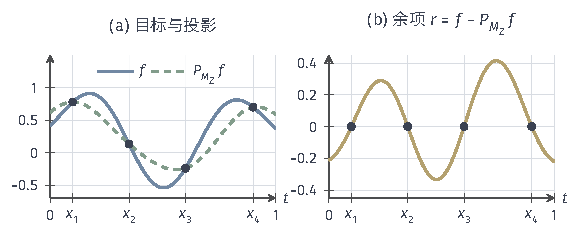
\includegraphics[width=97.9mm]{figures/02-abstract-mathematics/03-function-spaces/tikz/c5-observation-residual/figure.pdf}
  \caption{高斯核（$\sigma=0.15$）空间中的观测投影。(a)~目标$f=K_{0.2}-0.8K_{0.5}+0.9K_{0.8}$（实线）与它在$M_Z=\operatorname{span}\{K_{x_1},\ldots,K_{x_4}\}$上的投影（虚线），观测点$x_i=0.1,0.35,0.6,0.9$处两者取值相同（黑点）；(b)~余项$r=f-P_{M_Z}f$在每个观测点为零。读数只确定投影，余项对读数没有任何影响。}
  \label{fig:rkhs-observation-residual}
\end{figure}

\paragraph{Gram矩阵、读数与范数}

$M_Z$中的元素都能写成$g=\sum_ja_jK_{x_j}$，它的读数和范数都可以用Gram矩阵$\bm G_{i,j}=K(x_i,x_j)$计算：
\begin{equation}
\begin{gathered}
g(x_i)=\sum_ja_jK(x_i,x_j)=(\bm G\bm a)_i,\qquad
\|g\|_H^2=\bm a^{\top}\bm G\bm a,\\
\Bigl\langle\sum_ja_jK_{x_j},\sum_jc_jK_{x_j}\Bigr\rangle_H=\bm a^{\top}\bm G\bm c .
\end{gathered}
\label{eq:rkhs-gram-calculus}
\end{equation}
因此在$M_Z$内部，函数的全部计算都化为$n$维向量与$n\times n$矩阵的计算。注意$\bm a^{\top}\bm G\bm a$才是函数的范数平方，系数向量的欧氏长度$\|\bm a\|_2$一般与函数范数无关。

\paragraph{系数的不唯一与函数的不唯一}

有限观测下有两种不同的不唯一，它们来自不同的地方。第一种是系数的不唯一：两个系数向量$\bm a,\bm a'$给出同一个函数，当且仅当$\bigl\|\sum_j(a_j-a_j')K_{x_j}\bigr\|^2=(\bm a-\bm a')^{\top}\bm G(\bm a-\bm a')=0$，对半正定矩阵这等价于$\bm G(\bm a-\bm a')=\bm 0$。所以系数的冗余由$\ker\bm G$描述，它只是同一函数的不同写法。第二种是函数的不唯一：读数相同的函数可以相差$M_Z^\perp$中的任意元素，它们是真正不同的函数。

两个例子说明这两种情况互不决定。在仿射空间$H_{\mathrm{aff}}$中取$Z=\{-1,0,1\}$，第~\ref{sec:rkhs-kernel-properties}节已算出$\ker\bm G=\operatorname{span}\{(1,-2,1)\}$，系数不唯一；但三个核截面已经张成整个二维空间，$M_Z^\perp=\{0\}$，读数唯一确定函数。在$H_{\min}$中取$Z=\{1/3,2/3,1\}$，Gram矩阵
\[
\bm G=\frac13\begin{bmatrix}1&1&1\\1&2&2\\1&2&3\end{bmatrix},\qquad
\det\bm G=\frac1{27},
\]
可逆，系数唯一；但$M_Z^\perp$由在这三点取零的$H_{\min}$函数组成，是无限维的，读数远不能确定函数。若$K$严格正定，互异点上的Gram矩阵总可逆，第一种不唯一不会出现，第二种在无限维空间中却总是存在。

\subsection{有限中心的投影表示}
\label{sec:rkhs-center-projection}

上一小节说明读数确定$Pf$。现在把$Pf$实际算出来，即求出它在核截面$K_{x_1},\ldots,K_{x_n}$上的系数；这些观测位置在表示中充当中心。

\paragraph{正交条件与核矩阵方程}

设$Pf=\sum_ja_jK_{x_j}$。投影由正交条件$\langle f-Pf,K_{x_i}\rangle=0$（$i=1,\ldots,n$）刻画，由再生性质，它就是$(Pf)(x_i)=f(x_i)$，再由式~\eqref{eq:rkhs-gram-calculus}，
\begin{equation}
\bm G\bm a=\bm b,\qquad \bm b_i=f(x_i).
\label{eq:rkhs-center-equation}
\end{equation}
投影的正交条件与“在观测点插值”在这里是同一组方程。

\begin{theorem}[有限中心的投影]
\label{thm:rkhs-center-projection}
设$\bm b$是某个$f\in H$在$Z$上的读数。则：
\begin{enumerate}
\item 方程~\eqref{eq:rkhs-center-equation}有解，任意一个解$\bm a$都给出同一个函数$\sum_ja_jK_{x_j}=Pf$；
\item $Pf$是$M_Z$中唯一在$Z$上取读数$\bm b$的函数，也是$H$中所有满足$g(x_i)=\bm b_i$的函数$g$里范数最小的一个，且$\|Pf\|_H^2=\bm b^{\top}\bm a=\bm b^{\top}\bm G^{\dagger}\bm b$。
\end{enumerate}
\end{theorem}

\begin{proof}
$Pf\in M_Z$，可写成$\sum_ja_j^*K_{x_j}$，而$Pf$与$f$读数相同，所以$\bm G\bm a^*=\bm b$，方程相容。若$\bm G\bm a=\bm b=\bm G\bm a^*$，则$\bm a-\bm a^*\in\ker\bm G$，上一小节说明两组系数给出同一函数。对第2条，$M_Z$中两个读数相同的函数之差属于$M_Z\cap M_Z^\perp=\{0\}$。若$g\in H$满足$g(x_i)=\bm b_i$，则$g-Pf$在$Z$上取零，属于$M_Z^\perp$，勾股定理给出$\|g\|^2=\|Pf\|^2+\|g-Pf\|^2\ge\|Pf\|^2$。最后，$\|Pf\|^2=\bm a^{\top}\bm G\bm a=\bm a^{\top}\bm b$；取$\bm a=\bm G^{\dagger}\bm b$即得最后一个表达式。
\end{proof}

第1条区分了投影的唯一性与系数的唯一性。$\bm G$奇异时，可以用伪逆$\bm G^{\dagger}$从相容方程的全部解中选出欧氏长度最小的系数，这一性质可参考\BookChapterRef{chap:linear-equations-and-optimization}{卷一《数学准备：基础数学》“线性方程与矩阵方程”章中的伪逆与最小范数解}。但无论选哪一组系数，得到的函数都是同一个$Pf$；系数长度最小与函数范数最小是两回事，后者由第2条保证，与系数怎样选取无关。

\paragraph{最小值核的投影是折线插值}

在$H_{\min}$中，中心投影有一个直观的形式。取$Z=\{1/3,2/3,1\}$，$M_Z$由核截面$\min(\cdot,1/3)$、$\min(\cdot,2/3)$、$\min(\cdot,1)$张成，即在$1/3,2/3$处可以转折、左端为零的连续折线。由定理~\ref{thm:rkhs-center-projection}，$Pf$就是过原点和三个观测点的折线插值。以$f(x)=4x(1-x)$为例，读数为$\bm b=(8/9,8/9,0)$。折线在三段上的斜率依次为$8/3$、$0$、$-8/3$；而$\sum_ja_j\min(t,x_j)$在三段上的斜率依次为$a_1+a_2+a_3$、$a_2+a_3$、$a_3$，于是$\bm a=(8/3,8/3,-8/3)$。代回检验$\bm G\bm a=\bm b$：第一行$\tfrac13\cdot\tfrac83=\tfrac89$，第二行$\tfrac13\cdot\tfrac83+\tfrac23\cdot\tfrac83-\tfrac23\cdot\tfrac83=\tfrac89$，第三行$\tfrac89+\tfrac{16}9-\tfrac{24}9=0$。第~\ref{sec:rkhs-finite-features}节还会用到这个例子。

\paragraph{读数之外的误差}

投影在观测点上没有误差，那么在观测点之间误差有多大？由再生性质与$r\perp M_Z$，对任意$x\in X$，
\[
f(x)-(Pf)(x)=r(x)=\langle r,K_x\rangle=\langle r,K_x-PK_x\rangle ,
\]
第三个等号是因为$PK_x\in M_Z$与$r$正交。由Cauchy--Schwarz不等式，
\begin{equation}
|f(x)-(Pf)(x)|\le P_Z(x)\,\|f-Pf\|_H\le P_Z(x)\,\|f\|_H,
\label{eq:rkhs-power-bound}
\end{equation}
其中$P_Z(x)=\|K_x-PK_x\|_H$。
称$P_Z$为观测点组$Z$的\term{核插值幂函数}（power function）。它只依赖于核与观测位置，不依赖于目标函数：$P_Z(x)$是核截面$K_x$中不能被观测子空间表示的部分的长度。

$P_Z$可以用核矩阵算出。$PK_x$本身是一个投影，它的读数就是$K_x$的读数$\bm k_Z(x)=(K(x_1,x),\ldots,K(x_n,x))^{\top}$，由定理~\ref{thm:rkhs-center-projection}，$\|PK_x\|^2=\bm k_Z(x)^{\top}\bm G^{\dagger}\bm k_Z(x)$，再由勾股定理，
\begin{equation}
P_Z(x)^2=K(x,x)-\bm k_Z(x)^{\top}\bm G^{\dagger}\bm k_Z(x).
\label{eq:rkhs-power-function}
\end{equation}
在观测点$x=x_i$处，$K_{x_i}\in M_Z$，所以$P_Z(x_i)=0$。图~\ref{fig:rkhs-power-function}画出前一个高斯核例子的幂函数：它在四个观测点处为零，在相邻观测点之间隆起；间隔越大或离观测点越远，隆起越高，最大值约为$0.59$，出现在区间端点附近和$x_3,x_4$之间。同一图中，余项$|r(x)|$始终位于上界$P_Z(x)\|r\|_H$之下（这里$\|r\|_H=0.911$）。对最小值核，$K_x-PK_x$是$\min(\cdot,x)$减去它的折线插值，在$x$所在的小区间$[x_{k-1},x_k]$上是一个三角形，直接计算导数的平方积分得$P_Z(x)^2=(x-x_{k-1})(x_k-x)/(x_k-x_{k-1})$（约定$x_0=0$）。

\begin{figure}[!htb]
  \centering
  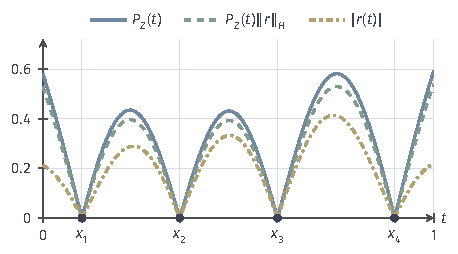
\includegraphics[width=77.5mm]{figures/02-abstract-mathematics/03-function-spaces/tikz/c5-power-function/figure.pdf}
  \caption{高斯核（$\sigma=0.15$）、观测点$x_i=0.1,0.35,0.6,0.9$的核插值幂函数$P_Z(t)=\|K_t-PK_t\|_H$（实线），以及图~\ref{fig:rkhs-observation-residual}中余项的绝对值$|r(t)|$（点划线）与上界$P_Z(t)\|r\|_H$（虚线，$\|r\|_H=0.911$）。幂函数在观测点处为零，只依赖于核与观测位置；余项总在上界之下。}
  \label{fig:rkhs-power-function}
\end{figure}

\paragraph{观测子空间自身的再生核}

前面处理的是一个给定函数的投影。换一个角度，观测子空间$M_Z$连同$H$的内积本身也是一个RKHS：对$g\in M_Z$，$g(x)=\langle g,K_x\rangle=\langle g,PK_x\rangle$，所以它的核截面是$PK_x$，再生核为
\begin{equation}
K_Z(x,z)=\langle PK_z,PK_x\rangle_H=\bm k_Z(x)^{\top}\bm G^{\dagger}\bm k_Z(z).
\label{eq:rkhs-projected-kernel}
\end{equation}
第二个等号用了$PK_x=\sum_jc_j(x)K_{x_j}$、$\bm c(x)=\bm G^{\dagger}\bm k_Z(x)$，以及式~\eqref{eq:rkhs-gram-calculus}和$\bm G^{\dagger}\bm G\bm G^{\dagger}=\bm G^{\dagger}$。同理，余下的$K-K_Z$是$M_Z^\perp$的再生核，因而也半正定，它的对角值就是$P_Z(x)^2$。

式~\eqref{eq:rkhs-projected-kernel}可以写成有限特征的内积。设$\bm G=\bm U\bm\Lambda\bm U^{\top}$是谱分解，$r$个正特征值组成$\bm\Lambda_r$，相应的特征向量组成$\bm U_r$。令
\[
\Phi_Z(x)=\bm\Lambda_r^{-1/2}\bm U_r^{\top}\bm k_Z(x)\in\mathbb R^r ,
\]
则$\Phi_Z(x)^{\top}\Phi_Z(z)=\bm k_Z(x)^{\top}\bm U_r\bm\Lambda_r^{-1}\bm U_r^{\top}\bm k_Z(z)=K_Z(x,z)$。$\Phi_Z$的第$k$个分量是函数$e_k=\lambda_k^{-1/2}\sum_j\bm U_{j,k}K_{x_j}$在$x$处的值，这些$e_k$构成$M_Z$的标准正交基：由式~\eqref{eq:rkhs-gram-calculus}，$\langle e_k,e_l\rangle=\lambda_k^{-1/2}\lambda_l^{-1/2}\bm u_k^{\top}\bm G\bm u_l=\delta_{k,l}$。

这里要分清两种近似。$Pf$近似的是一个给定的函数，误差取决于该函数的余项；$K_Z$近似的是核本身，它同时为$M_Z$中的所有函数提供再生关系，误差$K-K_Z$不涉及任何目标函数。式~\eqref{eq:rkhs-power-bound}把两者联系起来：给定函数的逐点误差不超过核误差的对角平方根乘以该函数的余项范数。中心应当怎样选取、读数带有噪声时采用什么拟合目标与惩罚、所得问题的解是否存在，都需要另外加入目标与观测模型；以核矩阵为工具的正则化回归可参考\BookChapterRef{chap:regression}{卷七《模型：经典模型》“回归”章中的核岭回归}，按样本抽取中心的低秩近似可参考\BookChapterRef{chap:dimensionality-reduction}{卷七“降维”章中的Nyström近似}。
